%% main.tex 
%% Main page of thesis complete package using MikTex 2.9 and TexStudio
%% 2015/10/05 
%% by Rizqiya Windy Saputra
%% contact me at rizqiya@students.itb.ac.id
%% for current contact information.
%%
%% Support sites:
%% https://www.sharelatex.com/
%% thanks to : 
%%		https://www.sharelatex.com,
%%		tex.exchange.com,
%%		stackoverflow.com,
%%		and Many other references were taken from google search.
%% ----------------------------------------------------------------


\documentclass[12pt]{report}
\usepackage[utf8]{inputenc}
\usepackage[english]{babel}

%% font
\usepackage{times} %%times new roman
%%\addto\captionsenglish{\renewcommand{\chaptername}{Lecture}}  %untuk mengganti nama judul setiap chapter

%% memasukan gambar ke document
\usepackage{float}
\usepackage{graphicx}
\graphicspath{ {images/} }

%% package untuk mengatur layout
\usepackage{fancyhdr}
\pagestyle{fancy}
%%\fancyhead[LE]{\slshape \rightmark} %section
%%\fancyhead[RE]{\thepage}
%%\fancyhead[RO]{\slshape \leftmark} % chapter
\fancyhead[L]{}
\usepackage{lipsum}
\usepackage{pdflscape}

%% membuat komentar panjang
%% memasukan komentar yang panjang
\usepackage{comment} %% pakai syntax \iffalse ---- \fi 
%%cara lain memberi comment
\usepackage{verbatim} %% bisa pakai \begin{comment} ---- \end{comment}
\iffalse  
%%ini bagian komentar,,\begin{comment}....\end{comment} tidak berfungsi pada bagian environment
%%cara pertama ini merusak posisi dari list of table, jadi tidak dalam satu halaman masing-masing, tapi bisa diakali dengan \newpage
	\usepackage{tocloft}
	\setlength{\cftfignumwidth}{3.5em}
	\setlength{\cfttabnumwidth}{3.5em}
\fi 
%% --- cara lain
%%untuk mengatur jarak pada penomoran list of figure, agar tidak dempet
\usepackage[titles]{tocloft}
\cftsetindents{figure}{0em}{3.5em}
\cftsetindents{table}{0em}{3.5em}

%% numbering gambar/table agar sesuai dengan judul di setiap subsection
\usepackage{amsmath}
\numberwithin{figure}{section}
\numberwithin {figure}{subsection}
\numberwithin {table}{section}
\numberwithin {table}{subsection}

%%\fancyfoot[]{\thepage}
\usepackage[a4paper,width=150mm,top=30mm,bottom=30mm]{geometry}
\renewcommand{\headrulewidth}{0.4pt} %% memberi baris pada header dengan ukuran 0.4pt

%% memberi spasi untuk judul 
\usepackage{setspace}
\usepackage{titlesec}
\onehalfspacing

%% mengurangi spasi di enumerate
\usepackage{enumitem} %% dalam dokumen nanti tinggal tambahain [nolistsep] setelah \begin{enumerate} 
%% cara ini ga kepake sih, karena menghilangkan space seluruhnya, tapi bisa dicoba akali dengan membuat \renewcommand

%% package untuk meletakan judul Bab di tengah
\usepackage{sectsty} 
\chapterfont {\centering} %% centering chapter
%%\sectionfont {\centering} %%section center
\setcounter{secnumdepth}{3} %% angka pada subsubsection

%% Mengatur Table kolom dan baris, merge, colouring dll
\usepackage{array}
\usepackage{multirow}
\usepackage[table]{xcolor}

%% Memberi indent untuk paragraph pertama
\usepackage{indentfirst}
\setlength\parindent{30pt}

%% Memasukan referensi
\usepackage[hyphens]{url} %%ditambahkan agar link url muncul di referensi

%%daftar singkatan
\usepackage[acronym, nopostdot,nonumberlist,toc]{glossaries}
\usepackage{acronym}
\makeglossaries
\loadglsentries{glossary.tex}

\begin{document}
\begin{titlepage}
\begin{center}
	\vspace{1cm}
	\large
		\textbf{SMART DISASTER MANAGEMENT BASED ON SERVICE SYSTEM ENGINEERING}\\
	
	\vspace{3cm}
	\textbf{THESIS}
	
	\normalsize
		\textbf{A Thesis Submitted in Partial Fulfillment\\
		for the Degree of Magister from\\
		Bandung Institute of Technology}
	
	\vfill
	\large
		\textbf{Rizqiya Windy Saputra}\\
		\textbf{23513146}\\
		\textbf{Magister of Informatics Study Program}
	
	\vspace{1cm}
	\includegraphics[scale=0.2]{logo-itb.jpg}
	
	\large
		\textbf{BANDUNG INSTITUTE OF TECHNOLOGY\\
		April, 2017}
\end{center}
\end{titlepage}
\cleardoublepage

%% The Front Matter
\clearpage
\pagenumbering{roman}
\chapter*{ABSTRACT}
\addcontentsline{toc}{chapter*}{ABSTRACT}
\begin{center}
	\large
		\textbf{INTELLIGENT DISASTER MANAGEMENT BASED ON SERVICE SYSTEM ENGINEERING}\\
	\vspace{0.5cm} %% memberikan spasi
	\normalsize
		\textbf{Rizqiya Windy Saputra}\\
		\textbf{23513146}\\
		\textbf{Magister of Informatics Study Program}
\end{center}

	Indonesian government using Hyogo Framework for Action (HFA) since January 2005. HFA is a global blueprint for 10-year plan to make the world safer from disaster losses. Since the implementation, Indonesia still has many challenges in developing Disaster Management (DM) Framework based on HFA. As one of many countries with disaster vulnerability, government aims to increase the resilience for their country. One of the ways is to deliver the value of Disaster Management to the communities by services provided. Service System Engineering (SSE) is growing faster now days. In this research, the DM Framework will be provided with the combination of SSE and HFA. SSE can be explain as individual and functional systems are linked together to define new meta-model system that can improve robustness, lower cost and increase reliability from Disaster Management. As the result, the research will provide the Architecture of Disaster Management that suitable for using in Indonesia.
%%\chapter*{Dedication}
%%thanks to ...
%%\chapter*{Acknowledment}
%%thanks to ....
\doublespacing

\tableofcontents
\addcontentsline{toc}{chapter}{Contents}
\listoftables
\addcontentsline{toc}{chapter}{List of Tables}
\listoffigures
\addcontentsline{toc}{chapter}{List of Figures}

\glsaddall
\printglossary[title={List of Terms}] %% makeindex thesis.glo -s thesis.ist -t thesis.glg -o thesis.gls
\printacronyms[title=List of Abbreviations] %% makeindex -s thesis.ist -o thesis.acr thesis.acn ...>> pdflatex thesis.tex
\renewcommand*{\glossarypreamble}{\thispagestyle{fancy}}
\renewcommand{\bibname}{References}

%% The Body Matter
\newpage
\pagenumbering{arabic}
\renewcommand{\baselinestretch}{2.5}  %spacing 1,5
%%\titlespacing*{\chapter}{0pt}{0pt}{40pt}
\titleformat{\chapter}[hang] %% reformat the chapter 
{\normalfont\Large\bfseries\centering\vspace{-4cm}}{\chaptertitlename\ \thechapter:}{1em}{}
%% resize the font in section, subsection or subsubsection
\sectionfont{\large}
\subsectionfont{\small}
\subsubsectionfont{\normalfont\small}

\chapter{Introduction}
\section{Background}
The disaster is divided to two types. The first one is disaster caused by human behavior such as fires, accidents, terrorism and murder. The other one is disaster occurred because of factors of nature itself such as floods, earthquakes, tsunamis and volcanic eruptions. The threatening of disaster can happen anytime or anywhere, and humans  can not avoid the risk of disaster. The most likely thing to do is to reduce the impact/risk and prepare the community in facing the disaster. there are many ways was developed and researched to prevent or reduce disaster impact, One of them is using disaster risk management (Disaster Management).\par
In recent years, Indonesia is very close to the many disasters. In line with it, Indonesia also has a serious problem in disaster prevention. There are many problems caused Indonesia become disaster area easily. Indonesia has many rivers, many active volcanoes, high rainfall and social economical habit. In the city, likes Jakarta and Bandung, Indonesia has flood as main problem and in rural area such as village, Indonesia has drought, avalanche and volcanoes eruption.  National Agency for Disaster Management (BNPB) states that between 1996 to 2014 Indonesia has three main problem disaster, that are flood, tsunami and drought\cite{DataBNPB}. The United Nations International Strategy for Disaster Reduction (UN-ISDR) ranks Indonesia at sixth biggest, with a loss of US \$27.84 billions in economical damage in 1991 to 2005. The data is not including the giant Tsunami disaster in 2004 and in few years later, the losses number can increase more and more.\par

\begin{figure}[h!]
\centering
\includegraphics[scale=0.7]{StatistikBencana.png}
\caption{\small Comparison of numbers of disasters between 1815 to 2014\cite{DataBNPB}}
\label{fig:StatBen}
\end{figure}

In January 2005\cite{HFAConference}, Indonesia Government uses a 10-year plan to make the world safer from natural hazard. The framework was named by Hyogo for Action (HFA) Framework. Substantively, The framework is not the first introduced to the world, because before using HFA, some global communities used Yokohama Strategy and Plan for Safer World as a unique opportunity to promote systematic and strategic approaches at the national level to address vulnerability and reduce the risk to natural hazards. In his improvisation, HFA framework has fives important and priority actions as a global blueprint to reduce disaster losses by 2015 in lives, economic and environmentally assets of communities and country.\par
Therefore, this research purposed an intelligent model of Disaster Management based on service system. In line with Service System Engineering (SSE) is becoming the huge development research in providing the services, the system that will be created has many opportunity to achieve HFA Framework purposes. SSE services many sector in communities live, where economy is the main sectors. In disaster management content, SSE will service environmental assets of communities as main sector and country as the sub sectors. Some researchers are utilizing a socio-economic and technological perspective to investigate end-user (customer) interactions with government organization or agency by developing formal methodologies for value co-creation and productivity improvements\cite{Lopes2013}. Technological perspective can wipe off some mistake of communities habit in disaster mitigation, provide the best way of getting disaster information, economize the cost expended and help disaster management agency providing services better.\par

\section{Statements of Problems}
\label{sec:StateOfProblem}
According to national progress report on the implementation of HFA (2011-2013)\cite{Framework2013}, there are many problem in disaster management (DM) implementation. One of them is the lack of synchronization between DM-related and non DM-regulation, such as those related to investment and economic development. The problems come from disharmony in regulatory of framework between any levels in government. And it can postpone the  more effective integration of disaster risk considerations into sustainable development policies, planning and programming at all levels, with a special emphasis on disaster prevention, mitigation, preparedness and vulnerability reduction\par
\begin{comment}
	masalah yangmuncul:
	1. Rendahnya proses sinkronisasi DM-related and non DM-Regulation ... apa itu DM related dan regulation,,, contohnya dalam investment dan ekonomi
	emphasis = penekanan

\end{comment}

Another problem of disaster mitigation process came from the society or community. A variety of disasters in Indonesia almost always showing  the same attitude that is a condition of the reactive and unplanned spontaneous as shown by the various stakeholders and communities. Each disaster in Indonesia is almost always colored and followed by a process called as \textit{a milling process}\cite{Kusmiati}, that is a situation where people do not know how to act or respond to disasters because there are no clear guidelines to be or if any such guidelines are not relevant to the conditions faced by society. This part is taking important reason when the amount of victims become huge.\par

Huge areas give more challenges to analyze the proper system that we need. as known as Indonesia ia a archipelago country with five big islands and many small islands, and the problems become harder when the location is a small island and isolated. The helpful effort and victim rescue processes in rare area will be slow and very difficult to be reached in short time. And the last problem is the variety losing of early warning detection devices after being placed in the sea\cite{AlatTsunamiHilang}. Many reason referable to this problem, as one of it is coming from the lacking of disaster education were gave to the communities.\par 

\begin{enumerate}
\setlength{\itemsep}{1.5pt}
\setlength{\parskip}{1.5pt}
\item[1.] Providing disaster management system based on HFA.
\item[2.] Providing the engineering services based on disaster management created.
\item[3.] Combining the Engineering Services and Disaster Management. 
\end{enumerate}\par

\section{Objectives}
The Model of Disaster management provided in this research is a combination between client (customer) and provider of services. The clients in this context are all society or community live in Indonesia and the providers are government and National Disaster Agency. This research will utilize many service engineering concept. Therefore, the objective of this research is how to formulate the disaster management based on appropriate service system engineering and Hyogo for Action Framework concepts.\par

\section{Research Question}
the combining of five important actions in HFA with service system will be the main focus of development disaster management model. The model that will be evolved consist of many possible service system. Possible regulations in providing the management system will be included too but not in specific and complex area.\par

\section{Scope and Limitation}
The scope of this research that will be provided are:
\begin{enumerate}
\setlength{\itemsep}{1.5pt}
\setlength{\parskip}{1.5pt}
\item[1.] Providing Disaster Management Model based on Hyogo for Action Framework
\item[2.] Combining the Disaster Management Provided with Service System Engineering
\item[3.] prototyping the system in mobile application\par
\end{enumerate}

\section{Research Output}
The output this research are a model of disaster management and a prototype of disaster management system. Both of them based on service system engineering. The system will provide a quick responses concept before the disaster attack even when after the attack. This system hopefully will support many cities in Indonesia to solve their problem in providing a good disaster management and give another option in improvisation of theory and application for better disaster management.

\section{Writing Systematic}
The writing systematics in this thesis are consisted of five main part, there are:
\begin{enumerate}
\setlength{\itemsep}{1.5pt}
\setlength{\parskip}{1.5pt}
\item[1.] CHAPTER I Introduction, provides a brief overview of the research background, problem formulation, research objectives, problem definition, research output, as well as systematic discussion.
\item[2.] CHAPTER II Literature, contains the review of the literature, a literature review and reference point-references relating to the cases examined in this study.
\item[3.] CHAPTER III Research Methods, describes the research methodology used as well as the research workflow.
\item[4.] CHAPTER IV Analysis and Design, explains the stages of analysis and design solutions to problems that are based on a theory that has been studied.
\item[5.] CHAPTER V Implementation and Testing, discussed the test scenarios with the aim of reinforcing, proving analysis and design that has been done in Chapter IV as expected
\item[6.] CHAPTER VI Conclusions and Recommendations, the conclusions drawn from the process analysis and modeling systems. As well as the suggestions are expected for the development of research in the future.
\item [7.] REFERENCES, contains a collection of the materials and references used by the author during the making of this thesis statements.
\end{enumerate}

\chapter{Literature Review}
\section{Service System Engineering}
Service engineering is a topic that is being discussed in today's technological world. Various forms of information technology development has now led to the service (services). It is also the underlying desire of the writer to lift a research thesis that incorporates service engineering to produce a good disaster management.\par

\subsection{Services}
\label{sebsec: ServicesDefinition}
Services are activities that cause a transformation of the state of an entity (people, product, business, and region or nation) by mutually agreed terms between the service provider and the customer. Individual services are relatively simple, although they may require customization and significant backstage support (e.g., database, knowledge management, analysis, forecasting, etc.) to assure quality and timely delivery. \par
Many term used in service science to describe service system. In this research, we choose to use Service System Engineering(SSE) term in order to not make confuse. Service System Engineering is a multidisciplinary approach to manage and design value co-creation of a service system. It extends the holistic view of a system to a customer-centric, end-to-end view of service system design \cite{SSEDefinition}. In other meaning, the approaches define to engineer system of system that are linked together so that can improve robustness, lower cost and increase liability. \par
\begin{comment}
	servvis adalah segala bentuk aktivitas yang mengtranformasi atau meubah bentuk dari sebuah entitas seperti masyarakat, procukatau bisnis dengan sebuah bentuk kepercayaan bersama antara si penyedia service atu layanan dengan si kostumer.
	
	sedangkan rekayasa sistem layanan adalah pendekatan-pendekatan yang yang diberikan untuk mengatur atau mendesain sebuah nilai dari sebuah sistem layanan. atau boleh dikatakan sebuah pendekatan untuk merekayasa sebuah sistem layanan untuk mendepatkan  tingkat ketahanan sistem yang lebih baik, mengurangi biaya dan meningkatkan kekuatan sistem.
	
	liability artinya bertanggung jawab, kecenderungan atau kekurangan
\end{comment}

Service System Engineering (SSE) has two core concept. Lopez and Pineda (2013) mention two core concept of SSE are service Meta-Model and Service Systems Development Process (SSDP). Service meta-model comprised of nine types of system entities to help business challenge and to create the the service value chain among relevant stakeholders to co-create the value.\par
\begin{table}[H] 
\begin{center}
\caption{Service Meta Model}
\label{tab: TabelServiceMeta}
	\vspace{0.1cm}
\begin{tabular}{ |p{3cm}|p{9cm}| }
 \hline
 \textbf{Entity} & \textbf{Atributes}\\
 \hline \hline
 Customers & Features, attitudes, preferences, requirements \\
 \hline 
 Goals & Business, service, customer\\
 \hline
 Inputs & Physical, information, knowledge, constraint\\
 \hline
 Output & Physical, information, knowledge, waste, customer satisfaction\\
 \hline
 Process & Service provision, service delivery, service operation, service support, customer relationship, planning and control\\
 \hline
 Human Enablers & Service providers, support providers, management, owners organization, customers\\
 \hline
 Physical enablers & Enterprise, building, equipment, enabling technologies, furnishing, etc\\
 \hline
 Informatics Enablers & information, knowledge, methods, process and tools (MPTs), decision support, skill acquisition. \\
 \hline
 Environment &Political, economic, social, technological, environmental factors.\\ 
 \hline
\end{tabular}
\end{center}
\end{table}\par

Next step after defining the entities needed in the system is building the process. The process built should have concern to tier of services entities to realize the overall service system. Lopez and Pineda (2013) purposed The Service Systems Development Process (SSDP) develop the service. SSDP consists of several repeating life-cycle phases with required inputs and expected outputs for each phase to help understand the activities required for realizing service systems. The system engineering phases are evolved to adapt and improve systems engineering methodologies to address the nature of Service Systems. The figure \ref{fig:SSDP} will offered a model of SSDP.\par

\begin{figure}[H]
    \begin{center}
    \includegraphics[scale=0.7]{sed.png}
        \caption{Service System Development Project\cite{Lopes2013}}
        \label{fig:SSDP}
    \end{center}
\end{figure}

The SSDP will identify the required input activities that execute to discover and designing the potential service needed and help analyze the service systems from an end-to-end perspective. During the service strategy phase new services are identified based on end user needs, mass collaboration trends, technology trends, and/or government/organization strategies. The government or stakeholder can decides to pursue the development of the selected service systems based on an extensive socio-techno-economic feasibility study. Service Life Cycle Management (LCM) methodologies such as continuous service improvement are utilized to analyze and set service improvements, potential service enhancements and to identify new service concepts across all entity types. Service LCM also includes strategies for replacement or disposal of the service/service entities, if applicable.\par

\subsection{Service Oriented Architecture}
The term service is widely used in the context of business and information technology. It is commonly understood as a facility supplying some public demand\cite{Haubrock2007}. This implies that a service can be performed by different entities, i.e. a human being, an enterprise as well as a hardware or software device as long as the idea of a service consumer on the one and a service provider on the other side is valid.\par
A service is a provider/client interaction that creates and captures value\cite{Haubrock2007}. The term SOA refers to service creation, interaction, presentation, and integration infrastructure capabilities to build business-level software based on reusable components. While this definition originates from Information Technology, it refers to several different aspects and disciplines involved in this approach: business processes, design and usability. In another meaning, SOA is essentially a collection of services. These services communicate with each other. The communication can involve either simple data passing or it could involve two or more services coordinating some activity. Some means of connecting services to each other is needed\cite{DefinisiSOA}.\par

\begin{figure}[H]
\centering
\includegraphics[scale=0.7]{ServiceEgineeringFramework.png}
	\caption{Service Engineering Framework}
	\label{fig:SEFramework}
\end{figure}

%% paragraph di bawah masih perlu perbaikan, karena full copy paste 
The new layer of abstraction introduced with service orientation now bares the potential to bridge the communication gap between IT developers and experts using these services, introducing a new business process- driven approach. For disaster management, this separation of concerns between definition and description of business processes and its actual implementation in form of computational services bares the potential to give consideration to the functional heterogeneity of partners involved. Public authorities or other institutions in disaster management are able to under- stand the semantics of the services and can therefore integrate them in their decision making process, while scientists and technicians provide and administrate these components.
SOA\par 

\subsection{Web Services}
Many of the benefits offered by the web service, especially high interoperability and the use that can be accessed anytime and anywhere as long as connected to the Internet network. Web service based on web standards and XML. web services discount significant role in SOA. Web services built upon protocols that already exist and have a platform independent, such as HTTP, XML, UDDI and WSDL. Those protocols provide services that can be found and used dynamically. SOA provides a service that has a contract that is platform independent interface, provided by XML. SOA emphasis on interoperability, it is provided by HTTP. This is what makes web services as the backbone of SOA.\par

\subsection{Unified Modeling Language}
Modeling is the designing of software applications before coding. Modeling is an Essential Part of large software projects, and helpful to medium and even small projects as well\cite{DefinisiUML}. A model plays the analogous role in software development that blueprints and other plans (site maps, elevations, physical models) play in the building of a skyscraper. Using a model, those responsible for a software development project's success can assure themselves that business functionality is complete and correct, end-user needs are met, and program design supports requirements for scalability, robustness, security, extendibility, and other characteristics, before implementation in code renders changes difficult and expensive to make. Surveys show that large software projects have a huge probability of failure - in fact, it's more likely that a large software application will fail to meet all of its requirements on time and on budget than that it will succeed\cite{DefinisiUML}.\par
UML 2.0 defines thirteen types of diagrams, divided into three categories, Six diagram types represent static application structure, three represent general types of behavior and four represent different aspects of interactions,
\begin{enumerate}
\setlength{\itemsep}{1.5pt}
\setlength{\parskip}{1.5pt}
\item [1.]\textbf{Structure Diagrams} include the Class Diagram, Object Diagram, Component Diagram, Composite Structure Diagram, Package Diagram, and Deployment Diagram. 
\item [2.]\textbf{Behavior Diagrams} include the Use Case Diagram (used by some methodologies during requirements gathering); Activity Diagram, and State Machine Diagram.
\item [3.]\textbf{Interaction Diagrams}, all derived from the more general Behavior Diagram, include the Sequence Diagram, Communication Diagram, Timing Diagram, and Interaction Overview Diagram.
\end{enumerate}
\begin{figure}[H]
    \begin{center}
    \includegraphics[scale=0.4]{contohUML.jpg}
        \caption{Sample of Use-Case Diagram \cite{SampleOfSimpleUML}}
        \label{fig:use-caseDiagram}
    \end{center}
\end{figure}

\subsection{Geographic Information System}
A geographic information system (GIS) is a computer system for capturing, storing, checking, and displaying data related to positions on Earth’s surface\cite{DefiniGIS}. GIS can show many different kinds of data on one map. This enables people to more easily see, analyze, and understand patterns and relationships. With GIS technology, people can compare the locations of different things in order to discover how they relate to each other. For example, using GIS, the same map could include sites that produce pollution, such as gas stations, and sites that are sensitive to pollution, such as wetlands. Such a map would help people determine which wetlands are most at risk.\par 

GIS can use any information that includes location. The location can be expressed in many different ways, such as latitude and longitude, address, or ZIP code. Many different types of information can be compared and contrasted using GIS. The system can include data about people, such as population, income, or education level (\figurename{\ref{fig:DefinisiGIS}}). It can include information about the land, such as the location of streams, different kinds of vegetation, and different kinds of soil. It can include information about the sites of factories, farms, and schools, or storm drains, roads, and electric power lines.\par
\begin{figure}[H]
    \begin{center}
    \includegraphics[scale=0.3]{gis.jpg}
        \caption{Multiple Layers of GIS \cite{DefiniGIS}}
        \label{fig:DefinisiGIS}
    \end{center}
\end{figure}\par
\vspace{-1cm}
\subsubsection{Global Positioning System}
The Global Positioning System (GPS) is a satellite-based navigation system made up of a network of 24 satellites placed into orbit by the U.S. Department of Defense\cite{DefiniGPS}. GPS was originally intended for military applications, but in the 1980s, the government made the system available for civilian use. GPS works in any weather conditions, anywhere in the world, 24 hours a day. There are no subscription fees or setup charges to use GPS.\par
GPS satellites circle the earth twice a day in a very precise orbit and transmit signal information to earth. GPS receivers take this information and use trilateration to calculate the user's exact location. Essentially, the GPS receiver compares the time a signal was transmitted by a satellite with the time it was received. The time difference tells the GPS receiver how far away the satellite is. Now, with distance measurements from a few more satellites, the receiver can determine the user's position and display it on the unit's electronic map. A GPS receiver must be locked on to the signal of at least 3 satellites to calculate a 2-D position (latitude and longitude) and track movement. With four or more satellites in view, the receiver can determine the user's 3-D position (latitude, longitude and altitude). Once the user's position has been determined, the GPS unit can calculate other information, such as speed, bearing, track, trip distance, distance to destination, sunrise and sunset time and more.\par 


\subsubsection{Location Based Services}
Location based services (LBS) are services offered through a mobile phone and take into account the device’s geographical location\cite{DefiniLBS}. LBS typically provide information or entertainment. Because LBS are largely dependent on the mobile user’s location, the primary objective of the service provider’s system is to determine where the user is. There are many techniques to achieve this.\par 

Some of the most common LBS applications include local news, directions, points of interest, directory assistance, fleet management, emergency, asset tracking, location-sensitive building, and local advertisement.\par

\subsection{Internet of Things(IoT}
Internet of Things [IoT] is a prevalent technology that is being emerged in information technology today. Since 1991 when IoT was proposed by Kevin Ashton, several research works are carried out in the field of IoT and its relevant technologies. Internet of (IoT) is an integrated part of Future Internet and could be defined as dynamic global network infrastructure with self configuring capabilities based on standard and interoperable communication protocols where physical and virtual "things" have identities, physical attributes and virtual personalities and use intelligent interface and are seamlessly integrated into the information network\cite{IoTDefinition}.

\section{Disaster and Disaster Management}
\vspace{-0.5cm}
\subsection{Disaster}
The term disaster was defined in many definition, there are :
\begin{enumerate}
\item[1.] a serious disruption of the functioning of society, causing widespread human, material and enviromental losses which exceed the ability of affected society to cope using only its own resources\cite{EffisientDM}
\item[2.] an incident or series of incidents that threaten and disrupt the lives and livelihood caused by natural factors and/or non natural factors effected in human casualties, environmental damage loss property and psychological impact\cite{DefinisiBencanaBNPB}.
\item[3.] a severe disruption, ecological and psychosocial, which greatly exceed the coping capacity of the affected community\cite{DisasterDefinition}.
\end{enumerate} \par
\begin{figure}[H]
    \begin{center}
    \includegraphics[scale=0.5]{hazardBagan.jpg}
        \caption{Classification of hazard based on causes\cite{definisiHazard}}
        \label{fig:DefinisiHazard}
    \end{center}
\end{figure}
Every community has some coping resources to deal with accidents and emergencies. Coping resources are the individual and community skills, materials, equipment or services that can be used to meet the demands created by an incident. The health care sector forms an important part of this, from the self-administered treatments available at a pharmacy or a walk-in clinic, through the Emergency Medical Services and hospital emergency departments, to the special care provided by burn wards or other tertiary services\cite{DMModelGuideline}.\par
Disaster management aims to shift the threshold at which an impact becomes a disaster\cite{DMModelGuideline}. This is achieved through two main methods: decreasing the amount of damage an impact can cause and increasing the capability of the community?s coping resources to deal with any damage that does occur. Disaster management ensures a coordinated response to make the best use of the community?s coping resources. The long-term recovery of the community is also a basic part of disaster management.\par

Disaster management has become a very important area worth exploration in the last few years, primarily due to the large number of disasters occurring across the world. Disaster management involves coordinating a large number of emergency responders to rescue people and recover infrastructure. The environment in which the responders act is often hazardous and full of uncertainties. Disaster response requirements are often identified by several distinctive characteristics and factors relevant to managing them \cite{MASDIsaster} such as: 
\begin{enumerate}
\setlength{\itemsep}{1.5pt}
\setlength{\parskip}{1.5pt}
\item[1.]disaster overwhelms the available resources 
\item[2.]disaster response should be immediate,
\item[3.]disaster events are unpredictable
\item[4.]uncertainty and incompleteness of information and resources
\item[5.]need for information and communication, and
\item[6.]disaster recovery strategy to recover from secondary crisis. 
\end{enumerate}\par

\subsection{Disaster Management Framework}
Hyogo Framework for Action is a global blueprint for disaster reduction. HFA starts in January 2005 at the world conference on disaster reduction held in Kobe, Hyogo, Japan. The framework is a foundation to 10-year plan to make the world safer from natural hazard. HFA has five priorities, there are\cite{HFAConference}:
\begin{enumerate}
\setlength{\itemsep}{1.5pt}
\setlength{\parskip}{1.5pt}
\item[1.]Ensure that disaster risk reduction is a national and a local priority with a strong institutional basis for implementation.
\item[2.]Identify, assess and monitor disaster risks and enhance early  warning
\item[3.]Use knowledge, innovation and education to build a culture of  safety and resilience at all levels
\item[4.]Reduce the underlying risk factor.
\item[5.]Strengthen disaster preparedness for effective response at all levels.
\end{enumerate}\par
Five priorities action above is being the core concept to develop disaster management concept. The reason for choosing HFA as a framework is proven by Djalante and Thomalla (2011). They examined several framework to develop the resilience to disaster by various way and human organizations, and argue that HFA is the most comprehensive for building resilience.\par
Stanganelli (2008) did another research in HFA framework. He suggests a new pattern of risk management. In his suggestion, risk management run in linear sequences. Beginning with assessment followed by prevention and mitigation, and concluding with preparedness and emergency response\cite{PatternRiskManagment}. Combining government and disaster agency have been experimented in Mongolia\cite{EffisientDM}. They try to identify the implications of national and regional disasters and devise province and district level mitigation strategies\par

\begin{figure}[H]
\begin{center}
\includegraphics[scale=0.7]{common-emergency.jpg}
\caption{Common Emergency Cycle\cite{CommonEmg}}
\label{fig:emg-cycle}
\end{center}
\end{figure}\par

\section{Theoritical Review}
There are many other research about  service system engineering and disaster management. To build a good service, it is necessary how the plan before, develop and manage the infrastructure development, products and services from Disaster Management. Furthermore, this research will use the framework of IT services to generate Disaster Management based IT services. many problems come since Indonesia Used HFA as Disaster Risk Reduction (DRR) guide. The formation of BNPB (the national agency for disaster management) and Law 24/2007 on Disaster Management have been the key drivers for progress in DRR. However, we have also revealed that local stakeholders are progressing considerably slower and at vastly different rates compared with their national counterpart. An imperative now is to improve the capacity and capability of local actors to manage resilience. \par  
Services are activities that cause a transformation of the state of an entity (people, product, business, and region or nation) by mutually agreed terms between the service provider and the customer. Individual services are relatively simple, although they may require customization and significant backstage support (e.g., database, knowledge management, analysis, forecasting, etc.) to assure quality and timely delivery. Service System Engineering (SSE) has two core concept. Lopez and Pineda (2013) mention two core concept of SSE are service Meta-Model and Service Systems Development Process (SSDP). Service meta-model comprised of nine types of system entities to help business challenge and to create the the service value chain among relevant stakeholders to co-create the value.\par


\section{Research Gap}
The disaster management is research many times, and from the research gives many references too. Although the research issued in social and behaviour issue. Service engineering is research many times too, and one of many paper provides the reference about the many application can be used in implementation of it. The Development of a model to investigate the disaster management system performance on the evacuation operation by employing different city with evacuation strategies. We reported our recent work on two major evacuation strategies, Demand Strategies (DS) and Speed Strategies (SS) which provide significantly improved evacuation results in smart cities settings. The future work will focus on further analysis and validation of additional disaster evacuation strategies.\par


\chapter{Research Methodology}
\section{Research Design}
\label{sec:ResearchDesign}
This research will use Design Research methodology (DRM) methodology. As stated by Lucienne T.M Blessing and Amaresh Chackrabarti in DRM, a Design Research Methodology book, this research proposal will using the step as DSRM framework, and Review based Comprehensive study approach:
\begin{figure}[H]
	\centering
    \includegraphics[scale=0.5]{DRMFramework.jpg}
        \caption{DRM Framework\cite{DRM.Framework}}
        \label{fig:DRM.Framework}
\end{figure}\par

DRM consists of four phases: Research Clarification, Descriptive Study I(DS I), Prescriptive Study (PS) and Descriptive Study II as mentioned in  Fig. \ref{fig:DRM.Framework} shows the links between these phases, the basic means used in each phase and the main outcomes. The bold arrows between the phases illustrate the main process flow, the light arrows the many iterations.
\begin{enumerate}
\item[1.]Research Clarification\par
%%In this phase author will be doing Literature Review study, to make problem identification and motive. In this phase author try to answer what does the main goal of this research topcis? Who needs this research? Why this research important?
In this phase, this study is trying to find some evidence or at least indications that support the assumptions in order to formulate a realistic and worthwhile research goal. the study does so mainly by searching the literature for factors that influence problem clarification. Based on the findings, an initial description of the existing situation is developed, as well as a description of the desired situation, in order to make the assumptions underlying each of the descriptions explicit. Initial reference model, initial impact model, preliminary criteria and overall research plan can be included in this phase.
\item[2.]Descriptive Study I\par
%%After having a clear goal and focus, author will review the literature for more influencing factor to elaborate the initial description of existing situation.
The intention of this phase is to make the description detailed enough to determine which factor(s) should be addressed to improve problem clarification as effectively and efficiently as possible. The analysis of the empirical data reveals the typical characteristics of insufficient problem definition and shows that insufficient problem definition in the problem-clarification phase is related to a high percentage of time spent on modifications in next phase of the process. This part may include by reference model and success criteria.
\item[3.]Prescriptive Study\par
%%In this stage, researcher will increased understanding of existing situation to correct and elaborate initial description and raised it into desired Situation
in this phase, this study uses the increased understanding of the existing situation to correct and elaborate o initial description of the desired situation. This description represents the vision on how addressing one or more factors in the existing situation would lead to the realisation of the desired, improved situation. This can develop various possible scenarios by varying the targeted factor(s). the study decides to focus on improving the quality of the problem definition as the most promising factor to address. this phase will be included impact model, support evaluation and outline evaluation plan. 
\item[4.]Descriptive Study II\par
the last phase is to investigate the impact of the support and its ability to realise the desired situation. Most of important point in this phase is evaluation. So, evaluation plan, application evaluation, success evaluation and implications are included in this phase. 
\end{enumerate}\par

\section{Research Workflow}
From the explanation of \ref{sec:ResearchDesign}, this research stand by the workflow below (Fig. \ref{fig:LangkahPenelitian}): \begin{enumerate}
\item[1.] Problems Identification. this stage becomes the important thing to be solved in this research. In this stage, the lack of synchronization between DM-related and non DM-regulation will be one of main problem to solved (mentioned at section \ref{sec:ResearchDesign}).
\item[2.] Literature Review. In this stage, the researcher collects many references from journals, articles, books or any informations related to problems stated at stage before.
\item[3.] Analysis and Identifications Solutions. There are many possible technologies can be used to solve the problem. In this phase, the researcher is trying to analyze and identify the best solution to used. 
\item[4.] Designing Model. Carried out in accordance with the results of analysis of technology solutions. Followed by architectural design, database, and display systems.
\item[5.] Prototyping. This stage is the stage of making a prototype of the analysis and design that has been generated from the previous process. Implementation is done in accordance with the tools and programming language that has been set. Implementation will be done only simulated and not all features will be implemented.
\item[6.] Testing. Performed to validate the system design. Tests conducted triangulation, namely through the black-box testing, simulation testing, and acceptance testing.
\item[7.] Evaluation. This stage is to look at the whole process of research and testing results to determine the conclusions of this study. Various suggestions may emerge from this evaluation stage.
\end{enumerate}\par
\begin{figure}[H]
\centering
\includegraphics[scale=0.6]{LangkahPenelitian.png}
\label{fig:LangkahPenelitian}
\caption{Research Workflow}
\end{figure}\par

\chapter{Analysis and Development}
\section{Analysis}
\vspace{-0.5cm}
\subsection{Current System Analysis}
\label{subsec:CurrentSystemAnalysis}
%% bahas  tentang kondisi real yang dihadapi, tambahkan alur layanan saat ini, proses-proses evakuasi(done),
%% sama layanan bisnis yang tersedia(done).
To build a good service, it is necessary how the plan before, develop and manage of infrastructure development, products and services from Disaster Management. Planning, development and managing every processes and steps in reducing impact of disaster will reduce the victims directly.\par 
Indonesia Disaster Ecosystem is consist of 3 (three) main actors. They are the Government, Disaster Stakeholders and people (community). The government consist of local or national government that taking a part in disaster reduction. Stakeholders such as Indonesian Red Cross, Hospitals and disaster rescue team, and of course the communities are the main actors. As same as another country, Indonesian government has their disaster management model as shown in figure \ref{fig:idm_figure}. Recent condition, system is divided to three stages. Activity, phase and function. Each stage has important point.\par 
\begin{figure}[H]
\begin{center}
\includegraphics[scale=0.85]{idm.jpg}
\caption{Indonesian Disaster Management Today \cite{Framework2013}}
\label{fig:idm_figure}
\end{center}
\end{figure}

Disasters, both natural and man-made, can strike anytime or anywhere. There are two ways to overcome disasters: the first is preventing them from occurring, and second is having an emergency system and plan of operation prior to the occurrence of any crisis. In either approach, information technology plays an important role in crisis management. Disasters, like earthquakes, floods, etc. can cause large number of deaths, injuries and homeless people. Appropriate responses are needed in the form of allocating resources to handle the effects of disasters\par

In statement of problems, this research mentioned about the lack of DM-Regulation and Non-Regulation such as those related to investment and economic development. Disharmony in regulatory framework for Disaster Risk Reduction (DRR) also exists between different levels of government. Integration of DRR into sustainable development policies has been initiated through risk sensitive spatial planning and development plan, but they have not been widespread as people’s understanding of these issues is still limited.\par
Common perception of DRR and a common understanding of the way to mainstream DRR into development have also not been achieved. Many decision makers, including those at the executive and legislative branches of the government, still hold the opinion that disaster management is a matter of responding to disaster events, and therefore disaster policies and budget are more focused on disaster response and post-disaster recovery aspects. Another challenge is that the existing Disaster Risk Reduction (DRR) policies have not been implemented well and translated into capacity and institutional development. Many relevant policies have been formulated at the central level, but their implementation at the provinces and districts/cities have not been to the maximum. The existing government administration system still limits resources for disaster risk reduction.
Future\par 

\begin{figure}[H]
\begin{center}
\includegraphics[scale=0.6]{BMbeforeSOA.png}
\caption{Information and Evacution Model Process}
\label{fig:EvaModel01}
\end{center}
\end{figure}

The figure \ref{fig:EvaModel01} above explain familiar process. The circulation mitigation process started after after disaster happen. The sensors that implemented to detect the disaster coming warn the communities, usually we call this with early warning. The information converted from sensor received by disaster information center. the next step is the decision making. The Government is a main actor here. Their decision need to be quick and precise, and the information will be delivered to communities. The process of delivering information  stopped here. Next step are depending on the communities, if they achieved the information and/or being in far from disaster location, they will be safe.\par
Figure \ref{fig:EvaModel01} also explained that current system not directly include disaster stakeholders.  Another stakeholders here can be Indonesian Red Cross (PMI), National Rescue Team Agency (BASARNAS) or Another National Disaster Mitigation Agency. Most of them got the information by themselves. Usually, The information comes from news media or from other people. Lack of information received effected to time of helping process. The rescue team came late to evacuation area and does not have enough preparation in area. The problem could be worse if the disaster attacked rural area.\par 

\begin{figure}[H]
\begin{center}
\includegraphics[scale=0.5]{BMafterSOA.png}
\caption{Business Process After Adding Services}
\label{fig:BisnisMOdelSOA}
\end{center}
\end{figure}
\par

As mentioned in  first section, this paper limit the research  in defining services needed and strategy to provide the DMS based on HFA. in the first section, many problems mentioned after implementation of HFA. Based on that cases, there are four main point government should do:\par

\begin{enumerate}
\setlength{\itemsep}{1.5pt}
\setlength{\parskip}{1.5pt}
\item Handling during disaster events that must be expedited.
\item Disaster education should be given to the society equally before the disaster occurred.
\item Handling of disasters should be evenly distributed in each region.
\item The coordination between government, stakeholders and many disaster management agency should be better addressed.
\end{enumerate}\par

Smart Disaster Management System (SDMS) also can be realized without four points above. Nevertheless, Indonesia is a country with large archipelago. Accordingly, SDMS in Indonesia can be created by modeling combination of various system with understanding of socio-economic states, technological advances and government policy. The growth of service science is going on to engineering sciences too. The service engineering can not be separated today. In many research we find that service engineering has been implemented in many sectors. Accordingly, we try to implement the service engineering method to disaster management system in Indonesia.\par

Business process designed (figure \ref{fig:BisnisMOdelSOA}) by adding some new element. The main actor in business process is government. Stakeholders added as the new element in business process. They will take a part in process of mitigation. The Government connected them directly to communities by sharing information as fast as they did to communities. By doing this, stakeholders/ disaster agency will come to disaster area soon after getting information with good preparation.\par

The information delivered to stakeholders in not only a part of small info about disaster happen. The information of location should be include in that short information. The location given is part of services. Using GPS technology at mobile phone and the disaster area informed, disaster rescue team can arrived at the area precisely.\par 

\section{SWOT Analysis}
Business Process Model is designed needs further analysis, therefore it takes a SWOT analysis. SWOT analysis is an analysis of internal and external conditions of an organization\ business process which in turn will be used as the basis for designing the strategy and working program. Internal analysis includes assessment of the strength factor (Strength) and weakness (Weakness), while the external analysis includes assessment of the chance factor (Opportunities) and challenges (Threats) of an organization / business process\cite{ThesisKangTeguh}.\par 
\begin{figure}[h]
\centering
\includegraphics[scale=0.4]{SWOTAnalysis.png}
\caption{SWOT Analysis}
\label{fig:swot}
\end{figure}\par

%% sepertinya pada gambar analisa swot yang bagian opportunities perlu ditambahain opportunities untuk stakeholders dan disaster agency,,,, karena yang ada pun baru satu buah	

The strength and weakness, both are internal problems. The external problems are the opportunity and threats. From the figure \ref{fig:swot} we can define four main points from SWOT analysis. The strength of this system are lied at high amount of smart phone users, easy information accessed, and helping the government in giving disaster mitigation. The weakness comes from the dependency of system with internet connectivity. The dependency will be a problem in rural area of disaster location. In some condition, information can not be accessed. From internal analysis, the opportunity of system comes from easy access. The easy access of information by government will evolve their existing system. The last is the threats of the system. Main threats is from internet connection exactly. This problem mainly comes because of dependency with internet from system.\par 

\section{Service Oriented Analysis for Disaster Management}
Figure \ref{fig:SEFramework} explain 3 main step of designing the services. Thomas Erl (2006), detailed that 3 main steps to design a service, the detail steps mentioned in figure below:
\begin{figure}[H]
\centering
\includegraphics[scale=0.7]{desainSOA.png}
\caption{SOA Analysis Design\cite{ThesisKangTeguh}}
\label{fig:DesainSOA}
\end{figure}\par

The first process to design the service based on design by the figure \ref{fig:DesainSOA} its explained by the figure itself. This step includes many process, they are defining business requirement, automation system identification and defining model service candidates. Defining business requirement is the first step in SOA analysis. The process of defining produced business requirement (see subsection \ref{subsec:CurrentSystemAnalysis})and SWOT analysis as shown as in figure \ref{fig:swot}. Automation system in this system include in delivering warning information to communities, and the last step is  started by outlining the business process to make the candidates of application service, if the system needs a revision in the manufacture of candidate service then the designing process will go through steps of service revision.\par
A simpler framework used in this research are Service System Development Process (SSDP) and Service Meta Model (see section \ref{tab: TabelServiceMeta}). SSDP consisted of at least 18 activities which grouped into four iterative phases, they are Service Need/ Strategy/ Concept, Service Design and Development, Service Transition/ Deployment, Service Operation. Service meta-model comprised of nine types of system entities to help business challenge and to create the the service value chain among relevant stakeholders to co-create the value (Fig. \ref{fig:MetaModelFig}).\par

\begin{figure}[H]
\begin{center}
\includegraphics[scale=0.8]{serviceMetaModel}
\caption{Service Meta-Model Entities \cite{Lopes2013}}
\label{fig:MetaModelFig}
\end{center}
\end{figure}\par

The figure \ref{fig:MetaModelFig} above gives easy steps to achieve a service goal. As this research aimed to achieve the same goal, combination of both, service meta model and Hyogo for Action Framework are an opportunity. Developing the smart system to support the disaster mitigation is part of using knowledge, innovation and education to build a culture of  safety and resilience at all levels.\par 
 
The figure \ref{fig:MainPartDM} below, represent main points of disaster management entities. The customer in SDMS should be communities, government and many agencies. The SDMS will receive various inputs from these customers with varying access. The inputs such as customer demands, mental and physic injuries and public safety. We defined customer demand as people or community need when disaster happen. The main need was defined from people area fast warning (early warning) and safe location for evacuation. The government also need to prepare any mental or physical damage at disaster victims. \par 

All customer providing mentioned at paragraph above will be define in the system. From these inputs and customer attributes, SDMS will create the service value chain that will make linkage between secondary part of SDMS. The value of service defined as output from the system. The outputs are customer demand fulfilled, safe customer (people), optimum disaster management and reconstructions and rehabilitations process working fast.\par

\begin{figure}[H]
\begin{center}
\includegraphics[scale=0.7]{idms.png}
\caption{Main Part of Disaster Management Based on Service}
\label{fig:MainPartDM}
\end{center}
\end{figure}\par

%gambar perlu dijelaskan secara terperinci dan jelas setiap bagian-bagiannya.
The important things of this phase are different communities condition and purposes. people lives in Sumatera island, most of them lives in rural area, and people lives in Java island lives in density area. In consequence, people in Sumatera can mitigate from disaster easier than people in Java. Different approach of area problem  will give solution to identify, asses and monitor disaster risk and enhance early warning system. \par
Secondary part of SDMS are utilizing, executing, monitoring and analyzing. SDMS should be using human enabler, physical enabler and information enablers. Many data from three of them will help SDMS to monitor and analyze environment. Furthermore, executes the processes.\par
 
\subsection{Business Process Identification}
As identification process is an important start to define the form of desired service to be delivered to community. To iterate, the purpose of service innovation is to improve value for communities. Therefore in the identification process there is must be a process to identify potential service of increasing the value, for this process we need a Business Model Canvas (BMC)\cite{SOASImple}. BMC can provide an overview of the Government to identify sector to improve in order to increase the value proposition.\par

\begin{landscape}
\thispagestyle{empty}
\begin{figure}[H]
\centering
\includegraphics[scale=0.8]{ServiceBlueprint.png}
\caption{Service Blueprint Smart Disaster Management System}
\label{fig:ServiceBlueprint}
\end{figure}
\end{landscape}\par

From the figure \ref{fig:ServiceBlueprint}, there are 3(three) lines to separate the interaction each action,
\begin{enumerate}
\setlength{\itemsep}{1.5pt}
\setlength{\parskip}{1.5pt}
\item Line with yellow color, this shown the interaction of communities as user to the system itself. 
\item Line with red color, the line shown the interaction service of government and stakeholders or disaster agency.
\item Line with green color, the last line shown the interaction between  government and the communities.
\end{enumerate}

The services shown in figure \ref{fig:ServiceBlueprint} are:
\begin{enumerate}
\setlength{\itemsep}{1.5pt}
\setlength{\parskip}{1.5pt}
\item Registration, communities should do this process to help local government saving their information. In this process, user's email address, phone number and their exact location should be inputed. In main condition, internet connectivity may be not work when disaster happen and for that reason, we need another option such as SMS.
\item Getting Disaster Information, People as user will get many disaster informations from mobile application. The informations was given by the government. 
\item Getting Disaster Warning, registered people will directly getting warned by mobile application when disaster happen. 
\item Getting Evacuation Route, the information achieved at registered people not only disaster warning but location of disaster happen. This is important part that evacuation route help people to evacuate precisely and directly without panic.
\item Looking for evacuation Location, this is additional option. People can see the evacuation point around his area. Infrastructure of evacuation point is another main aspect in disaster mitigation to be prepared.
\end{enumerate}

\subsection{Operation Candidates Identification}
In this part, We need to identify the operation candidates from the service blueprint that was designed. According to service blueprint, the operation candidates that possible in the system  are:
\begin{enumerate}
\setlength{\itemsep}{1.5pt}
\setlength{\parskip}{1.5pt}
\item evacuation route information, people can access information of route that will help them evacuate to right location.
\item evacuation location point. User also can access the information of evacuation location.  in future development, we can provide more information such as measure of building, building facilities or amount of evacuee.
\item registration process. Every user have to register their identity and choose different alias. People will register as community, government register as government and stakeholders or other disaster agency have to register as stakeholders. This difference is needed in parting the function in service.
\item Disaster warning notification. Showing the notification to evacuate as soon as possible when this notification coming.
\item Disaster agency information. Showing information of disaster agency or stakeholders that can help the victim in disaster time.
\item Government information. Showing government information, the details to be informed should be determined before.
\item user location. Showing user location information.
\end{enumerate}

\subsection{Logic Abstract Orchestration}
There are logic workflows separated from Both of Operation candidates identification and business process, there are:
\begin{enumerate}
\setlength{\itemsep}{1.5pt}
\setlength{\parskip}{1.5pt}
\item at the first step,user should register to login, if login process is successful user will be directed to main page.
\item if login was failed, user will be directed to choose two button. The first button is register button, and the second one is forgot password button.
\item email with registered user will not be working. 
\item not only email, phone number with registered user also will not be signed up for second time.
\item User can close the application when they finished read the information, and the application still run at back end.
\item User can check his location.
\item User also can ask some information they needed based on current disaster. 
\end{enumerate}

\subsection{Creating Service Candidates}
After getting candidates operation and logic abstract orchestration, the next step is creating service candidates as shown in figure \ref{fig:candidatesService} below:

\begin{figure}[H]
\centering
\includegraphics[scale=0.6]{candidatesService.png}
\label{fig:candidatesService}
\caption{Service Candidates}
\end{figure}

\subsection{Service Oriented Implementation and Repairing}
The step is repairing the service candidates that was made, but before jumping to it, a relevant Entity Relation Diagram (ERD) with the system must be defined. The defined ERD is shown in figure \ref{fig:ERDDiagram} below:\par

\begin{figure}[H]
\centering
\includegraphics[scale=0.6]{ERDDiagram1.png}
\label{fig:ERDDiagram}
\caption{Entity Relation Diagram}
\end{figure}

The explanation of ERD objects from the figure above are:
\begin{enumerate}
\setlength{\itemsep}{1.5pt}
\setlength{\parskip}{1.5pt}
\item Communities: an object represented people who need to be informed or warned when disaster is happening. In many conditions, user also can access some disaster informations given by government at application.
\item Government, an object represented the user account for government. The government user received disaster information from sensor systems to the application and share it if the information is dangerous and needed to be shared soon.
\item Stakeholders, an object represented as organization user account. The organization is taking a part in helping process after disaster attacking.
\item User Account, an object that represented all user in application. The users include communities, government and stakeholders.
\item Disaster Information, it represented to every information about disaster.
\item Evacuation Point, it represented the locatioan of disaster evacuation that the communities or disaster agency to be when the disaster happen. 
\end{enumerate}\par 

the relations between every entities in figure \ref{fig:ERDDiagram} could be explained in the table \ref{tab: TabelRelationEntity} below:
\begin{table}[h!] 
\begin{center}
\caption{Entity Relation Table}
\label{tab: TabelRelationEntity}
	\vspace{0.1cm}
\begin{tabular}{ |>{\centering\arraybackslash}m{2cm}|>{\centering\arraybackslash}m{3cm}|>{\centering\arraybackslash}m{3cm}|>{\centering\arraybackslash}m{3cm}|>{\centering\arraybackslash}m{3cm}|}
 \hline
 \textbf{Entity} & \textbf{Relation} & \textbf{Min Relation} & \textbf{Max Relation} & \textbf{Entity Name}\\
 \hline \hline
 Communities & accessed & 1 to 1 & 1 to 1 & Disaster Info\\
 \hline 
 Government & accessed & 1 to 1 & 1 to 1 & Disaster Info\\
 \hline
 Stakeholders or Disaster Agency & Accessted & 1 to 1 & 1 to 1 & Disaster Info\\
 \hline
 Evacuation Point & accessed & 1 to 1 & 1 to 1 &  Evacuation Point location\\
 \hline
\end{tabular}
\end{center}
\end{table}\par

After ERD process defined, service candidates can be redefined. Adaptability process is for completing service candidates identification process. service candidates that being adaptable is shown in figure below:

\begin{enumerate}
\setlength{\itemsep}{1.5pt}
\setlength{\parskip}{1.5pt}
\item Adding notification service as service candidate. 
\item Adding Disaster Info service as service candidate.
\item Adding detais informations from each type of user account.
\end{enumerate}

%% gabar perlu disesuaikan kembali
\begin{figure}[H]
\centering
\includegraphics[scale=0.7]{reidentifiedService.png}
\label{fig:ReServiceComposition}
\caption{Service Composition re-identified}
\end{figure}

\subsection{Service Composition Identification}
This step is to identify service candidates that have been made
previous to put in the orchestration layer, the business layer, or
the application layer. Figure \ref{fig:ServiceComposition} illustrates the composition identification service.

\begin{figure}[H]
\centering
\includegraphics[scale=0.6]{ServiceComposition.png}
\label{fig:ServiceComposition}
\caption{Service Composition}
\end{figure}

\subsection{Reviewing The Operation Candidates}
This step is reviewing the composition of the service that has been previously identified, Smart Disaster Management System, there are several services
which should be adjusted to be grouped into other services, including:

\subsection{Processing Analysis Needed}
SDMS business process is not complex, and it has identified all
candidate preparation service that illustrates the logic of the application. Therefore,
This step is not required in the SDMS.

\subsection{Application Service Operation Identification}
This step describe the process of service operation in the application, which is 
illustrated by the sequence diagram in figure :

\begin{enumerate}
\setlength{\itemsep}{1.5pt}
\setlength{\parskip}{1.5pt}
\item Sequence Diagram of authentication service
\begin{figure}[H]
\centering
\includegraphics[scale=0.5]{authenticationService.png}
\label{fig:AutService}
\caption{Authentication Service}
\end{figure}

\item Sequence diagram of utility services
\begin{figure}[H]
\centering
\includegraphics[scale=0.4]{UtilityService.png}
\label{fig:UtiService}
\caption{Utility Services}
\end{figure}

\item Sequuence diagram of government service
\begin{figure}[H]
\centering
\includegraphics[scale=0.4]{GovernmentService.png}
\label{fig:GovService}
\caption{Government Service Diagram}
\end{figure}

\item Sequuence diagram of stakeholder service
\begin{figure}[H]
\centering
\includegraphics[scale=0.5]{StakeholdersService.png}
\label{fig:StkService}
\caption{Stakeholder and Disaster Agency Service}
\end{figure}

\item Sequuence diagram of evacuation point service
\begin{figure}[H]
\centering
\includegraphics[scale=0.5]{EvacuationPointService.png}
\label{fig:EvaPointService}
\caption{Evacuation Point Service}
\end{figure}
\end{enumerate}

\subsection{Creating Application Service Candidates}
Identifications and specifications service design is needed to be changed to technical services, or usually known as application services or web services. The table 

\begin{table}[h!]
\begin{center}
\normalsize
\caption{Application Service Candidates}
\label{tab: AppServCand}
	\vspace{0.1cm}
\begin{tabular}{ |>{\centering\arraybackslash}m{1cm}|>{\centering\arraybackslash}m{3cm}|>{\centering\arraybackslash}m{5cm}|>{\centering\arraybackslash}m{3cm}|}
 \hline
 \textbf{No.} & \textbf{Application Service} & \textbf{Output} & \textbf{Parameters}\\
 \hline \hline
 1. & Login & success: boolean & username: string, password: string\\
 \hline 
 2. & CheckEmail & success: boolean & email: string \\
 \hline
 3. & AddUser & success: boolean & list $<$User Attribute$>$ \\
 \hline
 4. & GetDisInfo & List $<$DisInfoAttribute$>$ & code: string\\
 \hline
 5. & GetLocation & List $<$LocationAttribute$>$ & longitude: double, latitude: double \\
 \hline
 6. & GetEvaPointInfo & List $<$EvaPointAttribute$>$ & longitude: double, latitude: double  \\
  \hline
 7. & GetRoute & List $<$RouteAttribute$>$ & longitude: double, latitude: double  \\
  \hline
 8. & GetDisWarn & List $<$WarnAttribute$>$ & code: string \\
 \hline
 %%9. & GetDisInfo & 1 to 1 & 1 to 1 \\
 %%\hline
 %%10. & GetDisInfo & 1 to 1 & 1 to 1 \\
 %%\hline
\end{tabular}
\end{center}
\end{table}\par

%%\begin{comment}
%%\end{comment}


\subsection{Reviewing Service Compositions}
This step is the reviewing process of service compositions that was designed before. actually, for smart disaster management system, the compositions service was defined before and in consequence does not need to be reviewed.

\subsection{Reviewing Operation Candidates}
This step is also defined before, in consequence this step can be skipped to the next step.
\section{Service Oriented Designing}
\vspace{-0.5cm}
\subsection{Composing SOA}
As mentioned in this research, SOA in an element to develop the smart disasteranagement system. There 3(three) parts in composing SOA, selecting service ayerdefining the core standard and the last is selecting SOA extension. Each part of them wil be explained below.

\subsubsection{Service Layer Selecting}
There are 3(three) layers to be used in this SOA composing. Orchestration layer, business layer and application layer. All of them have been explained before in figure \ref{fig:ServiceComposition}.

\subsubsection{Core Standards Position}
This step is core standard designing step. The design will be used in web service. The figure below is shown the core standard used in smart disaster management system.

\subsubsection{SOA Extension Selecting}
SOA extension that will be used in SOA composing is WS-sdms.

\section{Application Designing}
The prototype will be build to support the system. The prototype is going to build in mobile application and web application that used every services explained before. This explanation focused at architecture function and design function fro the system built. The development will follow the business process step and SOA design that defined before.\par  
Designing of structure and function will be defined by use case diagram, and user interface will created for mobile application and web application. There areany ways to create the application, but in this research the easiest part will be used. Application will be built using HTML 5. In addition as easy programming, HTML 5 is also based on web application, so it will help us when the application needs the maintenance. The compatibly of HTML 5 with many devices is also a reason in creating this application.The compatibly of HTML 5 is shown at figure \ref{fig:html5}. \par 

\begin{figure}[H]
\centering
\includegraphics[scale=0.25]{html5.png}
\label{fig:html5}
\caption{The Compatibly of HTML 5 with Web Applications \cite{HTML5}}
\end{figure}

\section{Use Case Diagram}
Use case diagram are determined on basic functions needed. Basic functions are defined in use case diagram is helping to make the application easier to understand and all needed will be accommodated in use case diagram. A next explanations will cover the explanations of use case diagram was defined.

\begin{enumerate}
\item User (Communities)\par 
community user account is main actor in this system. The community start using the application by login to it. After login, user can access disaster information, evacuation point information and getting warning notification.  
\begin{figure}[H]
\centering
\includegraphics[scale=0.4]{UserComDiagram.png}
\label{fig:comUseCase}
\caption{Community Use Case Diagram}
\end{figure}

The explanation of use case  diagram above is:
\begin{table}[H]
\begin{center}
\caption{Community Use Cases Diagram}
\label{tab: ComUCDiagram}
	\vspace{0.1cm}
\begin{tabular}{ |>{\centering\arraybackslash}m{2cm}|>{\centering\arraybackslash}m{4cm}|>{\centering\arraybackslash}m{6.5cm}|}
 \hline
 \textbf{Actors} & \textbf{Use Cases} & \textbf{Descriptions} \\
 \hline \hline
  (AK01) User Community & (UC01) Disaster Info & This function used for getting disaster information which that provided from government or from sensor system directly. \\
 \hline 
 & (UC02) Evacuation Point & This function used for searching the location of evacuation points. In some condition, evacuation points is depend on the government. \\
 \hline
 & (UC03) Disaster Warning & This function used for getting warning of disaster happen. Its also a warning to do evacuation process to user received the warning. \\
 \hline 
 & (UC04) Disaster Route This function used for user get best way to run when they get the warning to evacuate& \\
 \hline
 %%\hline
\end{tabular}
\end{center}
\end{table}

\item User (Government)\par
Government is has another initial user account. When register process, they will directed to choose as government. As the government, user will get disaster information and sent warning notification to both other user account (Community and Stakeholder).

\begin{figure}[H]
\centering
\includegraphics[scale=0.4]{UserGovDiagram.png}
\label{fig:govUseCase}
\caption{Government Use Case Diagram}
\end{figure}

The explanation of use case  diagram above is:
\begin{table}[H]
\begin{center}
\caption{Community Use Cases Diagram}
\label{tab: ComUCDiagram}
	\vspace{0.1cm}
\begin{tabular}{ |>{\centering\arraybackslash}m{2cm}|>{\centering\arraybackslash}m{4cm}|>{\centering\arraybackslash}m{6.5cm}|}
 \hline
 \textbf{Actors} & \textbf{Use Cases} & \textbf{Descriptions} \\
 \hline \hline
  (AK02) User Government & (UC05) Disaster Info & This function used for getting disaster information which that provided from government or from sensor system directly. \\
 \hline 
 & (UC06) Disaster Warning & This function used for sending the warning message to other two both user, community and stakeholders. \\
 \hline 
 %%\hline
\end{tabular}
\end{center}
\end{table}

\item User (Stakeholder)\par 
Stakeholder account actually same like community account. The difference between two of them is at limited service they get. Stakeholders account only get warning notification and evacuation point. Both are important in stakeholder.
\begin{figure}[H]
\centering
\includegraphics[scale=0.4]{UserStkDiagram.png}
\label{fig:stkUseCase}
\caption{Stakeholder Use Case Diagram}
\end{figure}

The explanation of use case  diagram above is:
\begin{table}[H]
\begin{center}
\caption{Stakeholders Use Cases Diagram}
\label{tab: stkUCDiagram}
	\vspace{0.1cm}
\begin{tabular}{ |>{\centering\arraybackslash}m{2cm}|>{\centering\arraybackslash}m{4cm}|>{\centering\arraybackslash}m{6.5cm}|}
 \hline
 \textbf{Actors} & \textbf{Use Cases} & \textbf{Descriptions} \\
 \hline \hline
  (AK03) User Stakeholders & (UC07) Disaster Info & This function used for getting disaster information which that provided from government or from sensor system directly. \\
 \hline 
 & (UC08) Evacuation Point & This function used for searching the location of evacuation points. In some condition, evacuation points is depend on the government. \\
 \hline
 & (UC09) Disaster Warning & This function used for getting warning of disaster happen. Its also a warning to do evacuation process to user received the warning. \\
 \hline 
 %%\hline
\end{tabular}
\end{center}
\end{table}
\end{enumerate}

All use cases are mentioned can be explained in one figure as shown as figure \ref{fig:MainUseCase}:
\begin{figure}[H]
\centering
\includegraphics[scale=0.5]{MainUseCaseDiagram.png}
\label{fig:MainUseCase}
\caption{Complete Use Cases Diagram of the System}
\end{figure}

\section{Technology Architecture}
This section will explain about technology used in service implementing process. There are different technology was used in developing, and which difference used was based on needed from the system.
\begin{enumerate}
\item Web base application. Using Service Oriented Architecture made the application need a web application in implementation. Its because between user interface at application can not be separated with the service available.
\item Short Message Service (SMS), event internet is the main technology today, we need a back up technology to support the application in rural area. Rural area is not only a reason for implementing the SMS, many people in local area still using SMS in main way of communicating each other.
\item Cloud Computing Technology. The familiar technology is used now days. Easy access in many ways for user. This technology help user to access the application with his smart phone, tablet, laptop or computer device. 
\end{enumerate}
The explanation above can be defining in figure \ref{fig:TechUsed}:
\begin{figure}[H]
\centering
\includegraphics[scale=0.6]{techUsed.png}
\label{fig:TechUsed}
\caption{Technology Architecture Used in Smart Disaster Management System}
\end{figure}


\begin{comment}
\begin{table}[h!]
\begin{center}
\caption{Application Service Candidates}
\label{tab: AppServCand}
	\vspace{0.1cm}
\begin{tabular}{ |>{\centering\arraybackslash}m{2cm}|>{\centering\arraybackslash}m{3cm}|>{\centering\arraybackslash}m{5cm}|}
 \hline
 \textbf{Actors} & \textbf{Use Cases} & \textbf{Descriptions} \\
 \hline \hline
  &  &  \\
 \hline 
 &  &  \\
 \hline
 &  &  \\
 \hline
 &  & \\
 \hline
 %%\hline
\end{tabular}
\end{center}
\end{table}\par
\end{comment}
\chapter{Result and Conclusion}
\section{Result}
\vspace{-0.5cm}
\subsection{System Implementation}
To determine the success of the system has been designed, The system has been implemented in software application that can be used with functions defined appropriately. The following is a discussion of the implementation of a software prototype development of Smart Disaster Management System.
\subsubsection{Implementation Environment}
Implementation of this system is using software and hardware environment. The mentioning of environment is important for maintenance process in future if we need upgrade or adding some new services. The hardware specifications are :
\begin{enumerate}
\setlength{\itemsep}{1.5pt}
\setlength{\parskip}{1.5pt}
\item Processor Intel Celeron 2.16GHz
\item RAM 2GB
\item Hard disk 500GB.
\end{enumerate}\par 

and the software specification are:
\begin{enumerate}
\setlength{\itemsep}{1.5pt}
\setlength{\parskip}{1.5pt}
\item Windows 10 Operating System x64bit
\item Notepad++ v6.9.1
\item Ionic mobile application framework
\item Node JS v4.5.0
\item Angular JS v1.5.8
\end{enumerate}

\subsubsection{Implementation Limit}
The Limit of developing smart disaster management system are:

\begin{enumerate}
\item Disaster information data provided by BMKG
\item The security of application is not part of discussion here 
\end{enumerate}

\subsubsection{Implementatiton Steps}

\subsubsection{Implementation Result}
\subsection{Testing Process}
\section{Conclusion and Suggestion}
\subsection{Conclusion}
\subsection{Suggestion}

%% The End Matter
%%\appendix 
%%\chapter{Appendix 1: Research Project Manager}
%%\section{Work Breakdown Structure}

\begin{table}[h!]
\centering
\caption{Table Appendix 1: Work Breakdown Structure}
\label{tab: app1}
\begin{tabular}[h!]{|p{6cm}|p{2cm}|p{2cm}|}
\hline
Task & Effort & Status \\
\hline
Problem Identification & 1 & done \\
\hline
Define the need of Disaster Management & 1 & done \\
\hline
Breakdown Service Engineering based on Multi Agent System & 2 & - \\
\hline
DMS Implementation & 3 & - \\
\hline
Evaluation & 3 & -\\
\hline 
\end{tabular}
\end{table}

\section{Schedule}
\begin{table}[h!]
\centering
\caption{Table Schedule of Work}
\label{tab: SchWork}
\begin{tabular}[h!]{|p{4cm}|p{0.2cm}|p{0.2cm}|p{0.2cm}|p{0.2cm}|p{0.2cm}|p{0.2cm}|p{0.2cm}|p{0.2cm}|p{0.2cm}|p{0.2cm}|p{0.2cm}|p{0.2cm}|p{0.2cm}|p{0.2cm}|p{0.2cm}|p{0.2cm}|p{1cm}|}
\hline
\multirow {2}{4em}{Task} & \multicolumn{4}{|c|}{First Month} & \multicolumn{4}{|c|}{Second Month} & \multicolumn{4}{|c|}{Third Month} & \multicolumn{4}{|c|}{Fourth Month} & \\
 & 1 & 2 & 3 & 4 & 1 & 2 & 3 & 4 & 1 & 2 & 3 & 4 & 1 & 2 & 3 & 4 &  \\
\hline
Problem Identification & V & V &  &  &  &  &  &  &  &  &  &  &  &  &  &  & done \\
\hline
Define Solution Objective &  &  & V & V &  &  &  &  &  &  &  &  &  &  &  &  &  \\
\hline
SOA Analysis and Development &  &  &  &  &  &  &  &  &  &  &  &  &  &  &  &  &  \\
\hline
SOA Implementation &  &  &  &  &  &  &  &  &  &  &  &  &  &  &  &  &  \\
\hline
Evaluation &  &  &  &  &  &  &  &  &  &  &  &  &  &  &  &  &  \\
\hline
\end{tabular}
\end{table}

%% Print halaman referensi
\bibliographystyle{unsrt}
\bibliography{referensi}
%%\bibliographystyle{plain}
\nocite{*}
\end{document}